\Chapter{A különböző rácsok a játékokban}

\section{Rácsok összehasonlítása}

Legyen szó társasjátékról vagy számítógépes játékról, az egyik leggyakrabban használt rács a négyzetrács. Egyszerű, könnyen kezelhető és jól illeszthető a számítógép kijelzőjére.
\newline A cellák pozícióit a Descartes-féle derékszögű koordináta-rendszer ($x, y$) segítségével határozhatjuk meg. 
\newline Kirajzolásához ismernünk kell a cella méreteit (szélesség, magasság) illetve a rács méreteit (oszlopok, sorok száma). 
\newline A nyilvántartáshoz ismernünk kell a viszonyítási pontot (origó), illetve tudnunk kell az objektum pozícióját ($x, y$).
\newline
\newline Könnyen kezelhetősége mellett viszont van egy nagy hátránya:
Egy négyzetnek nyolc szomszédja van. Oldalain keresztül vízszintesen, valamint függőlegesen 2-2 szomszédja érhető el. További négy szomszédja átlósan található meg. A problémára akkor figyelünk fel, amikor megvizsgáljuk a távolságot a különböző szomszédok között. A vizsgálathoz tegyük fel, hogy az oldalak hossza 1. Ha a négyzetek középpontjához viszonyítunk, akkor a függőlegesen és a vízszintesen lévő szomszédok távolsága 1, míg az átlósan lévők távolsága $\sqrt{2}$.
\newline

\begin{figure}[h]
\centering
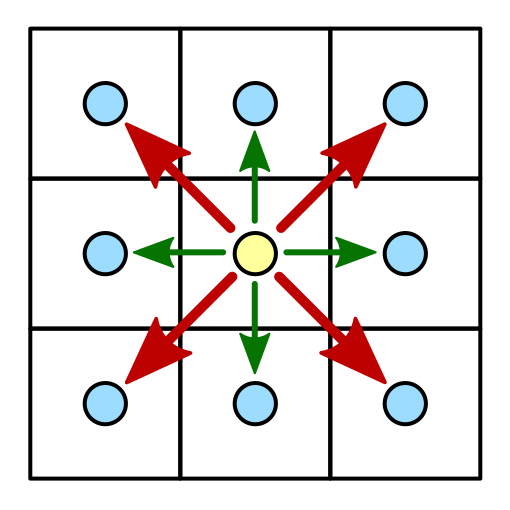
\includegraphics[scale=0.2]{kepek/img21.png}
\caption{A szomszédok távolsága a négyzetrács esetén}
\label{fig:img21}
\end{figure}

\noindent A két fajta szomszéd közötti különbség miatt vetődnek fel bizonyos kérdések:
\newline
\newline Hogyan kezeljük az átlós mozgást? 
\newline Egyáltalán engedélyezzük-e az átlós mozgást? 
\newline
\newline A problémára több megoldás is létezik:

\begin{itemize}
\item Nem alkalmazunk átlós mozgást. Ez a legegyszerűbb megoldás, amit az egyszerűsége miatt gyakran használunk.
\item Egy kevésbé elterjedt megoldás, hogy maradunk a négyzeteknél, viszont minden második sort/oszlopot eltolunk az oldal hosszának a felével. Ekkor az összes szomszéd hasonló távolságra kerül.

\begin{figure}[h]
\centering
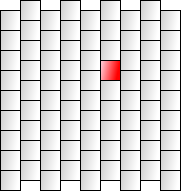
\includegraphics[scale=0.4]{kepek/img22.png}
\caption{Az Eltolásos négyzetrács}
\label{fig:img22}
\end{figure}

\item A leggyakoribb megoldás a hexagonok használata a négyzetek helyett. A négyzethez hasonlítva a hatszögnek csak hat szomszédja van (nyolc helyett). Ezek közül mindegyik oldal szomszéd, és nincs olyan szomszédja ami a sarkokhoz esne. Ezáltal minden szomszéd egyenlően 1 távolságra van.
\end{itemize}

\noindent A hexagonrácsot azért szokták játékokban használni mert kevésbé torzítják a távolságokat mint a négyzetrács. Ez azért van mert nincs átlós szomszédja ellentétben a négyzettel. (Az átlós szomszédok torzítják a távolságokat.)

\begin{figure}[h]
\centering
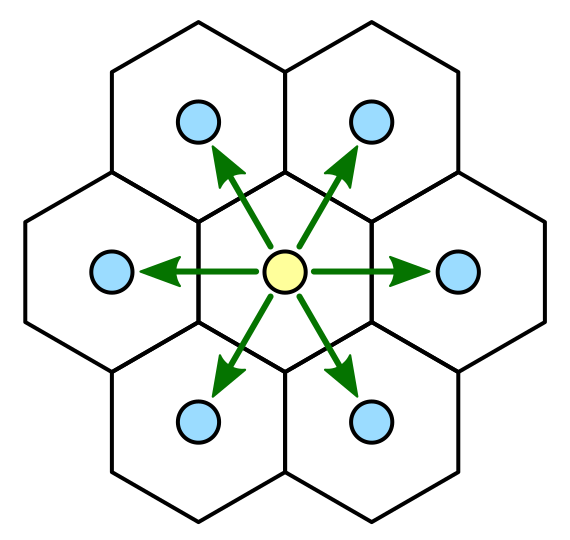
\includegraphics[scale=0.2]{kepek/img23.png}
\caption{A szomszédok távolsága a hexagonháló esetén}
\label{fig:img23}
\end{figure}

\noindent A fő indok a hexagonháló mellett az eltolt négyzethálóval szemben az, hogy sokkal kézenfekvőbb a hat lehetséges mozgási iránynak a használata. Emellett még esztétikailag is kellemesebb érzetet nyújt a felhasználó számára.

\section{Rácsok felhasználása}

Alapvetően mindkét rácsnak megvan a maga helye a játékfejlesztésben. 
\newline
\newline Mivel a beltéri helyszínek (szobák) és az azon belüli elemek (bútorok) általában téglalap alakúak, praktikusabb a négyzetrács használata. A négyzetrács a falakhoz tökéletesen illeszkedik, ugyanakkor a hexagonok esetében problémák merülnek fel. Ugyanis a hexagonok nem fognak szabályosan illeszkedni a falak mentén. Erre kétfajta megoldás létezik: a fal menti hexagonokat elvághatjuk, vagy másik megoldás, ha nem töltjük ki a fennmaradó helyeket. Egyik megoldással sem lehetünk maradéktalanul elégedettek, ha elvágjuk a hexagonokat. 
\newline

\begin{figure}[h]
\centering
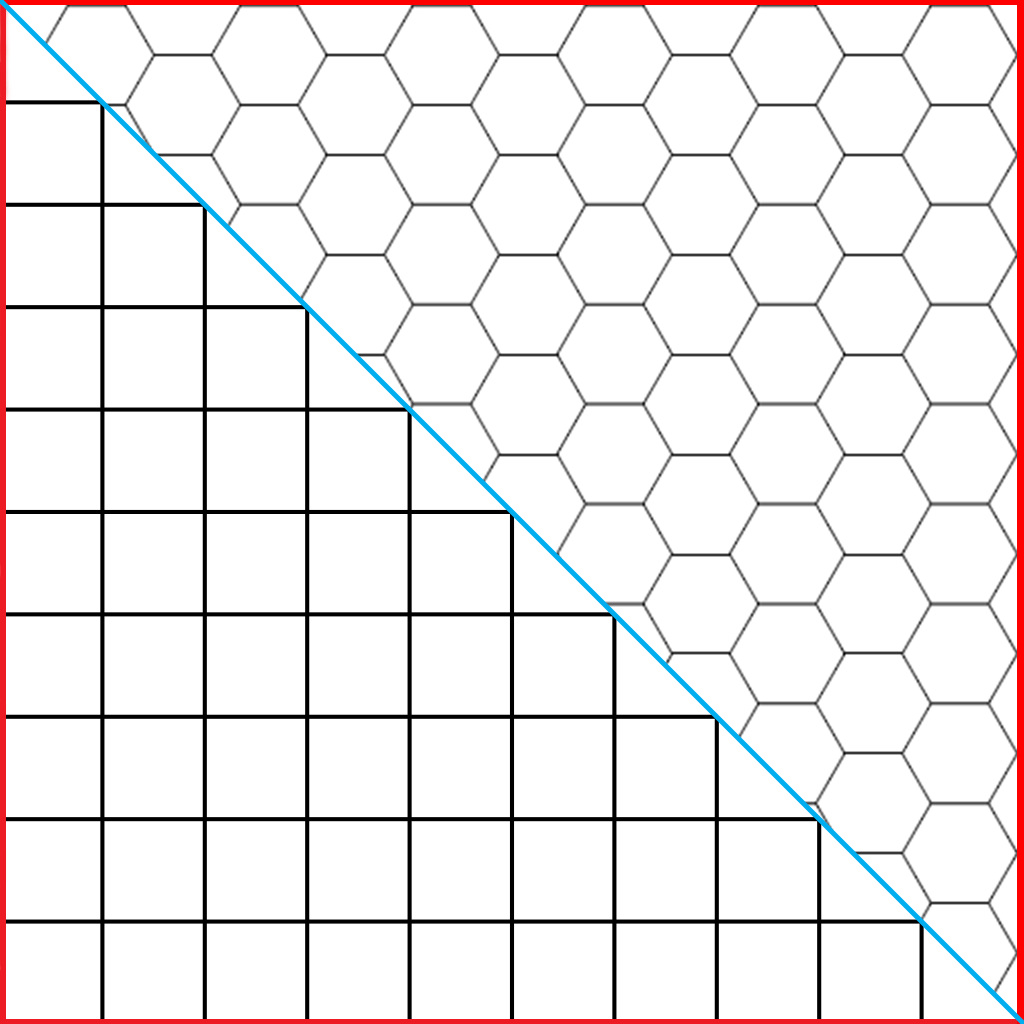
\includegraphics[scale=0.1]{kepek/img24.png}
\caption{A hexagon és a négyzet rács zárt térbeli összehasonlítása.}
\label{fig:img24}
\end{figure}

\noindent Akkor azok hogyan viselkedjenek? 
\newline Lehessen-e rálépni?
\newline Ha nem lehet rálépni akkor miért van?
\newline
\newline Ha csak kihagyjuk a széleken a hexagonokat amik nem férnek el az a felhasználó számára furcsa összhatást nyújthat.
\newline
\newline Ha mindenképpen hexagonokat  szeretnénk használni kis méretű térképen (pl: $8 \times 20$), akkor lehetőleg ne egy zárt szobában alkalmazzuk hanem szabad téren (pl: mező, erdő, tengerpart) vagy próbáljuk a hexagon rács széleihez igazítani a környezetet.
\newline
\newline Kültéren, falak hiányában ezek a problémák nem merülnek fel. Emiatt, valamint a négyzetrács átlós mozgásával kapcsolatos problémák miatt előnyösebb a hexagonháló használata ezekben az esetekben.

